\chapter{Preparation}

\section{Theory}

\subsection{Slab Waveguide}
\subsubsection{Calculation of Modes}
\subsubsection{Field Distribution and Dispersion Diagramm}


\subsection{Strip Waveguide}



\section{Questions}

\subsection{Slab and Strip waveguide?}
\label{q1}
% A waveguide usualy consists of a core material with a destinct refractive index surrounded by a cladding with another refractive index. For planar waveguides the lower layer is usualy called substrate. For guiding modes in the waveguide the refractive indices of the core has to be higher than the refractive indices of the cladding and substrate.
A slab waveguide consists of three lateral infinitly spread layers  with different refractive indices (cf. figure \ref{fig:}). In planar waveguide structures the upper layer is usualy called cladding, the middle layer core and the lower layer substrate. The strip waveguide also consists of these layers but the core is not infinitely spread (cf. figure \ref{fig:}). It rather has a destinct width in one direction. Thus the field is confined in two dimensions.

For guiding modes the refractive index in the core has to be higher than the refractive index in the cladding and the substrate. Common materials for a such waveguides are SiO$_2$ (n $\approx 1.47$) as Substrate, Si (n $\approx 3.5$) as core and some Polymere (n $\approx 1.5$) as cladding.

\subsection{Different performance between TE and TM @ boundary}

\subsection{Single Mode strip waveguide}

\begin{figure}%
\centering
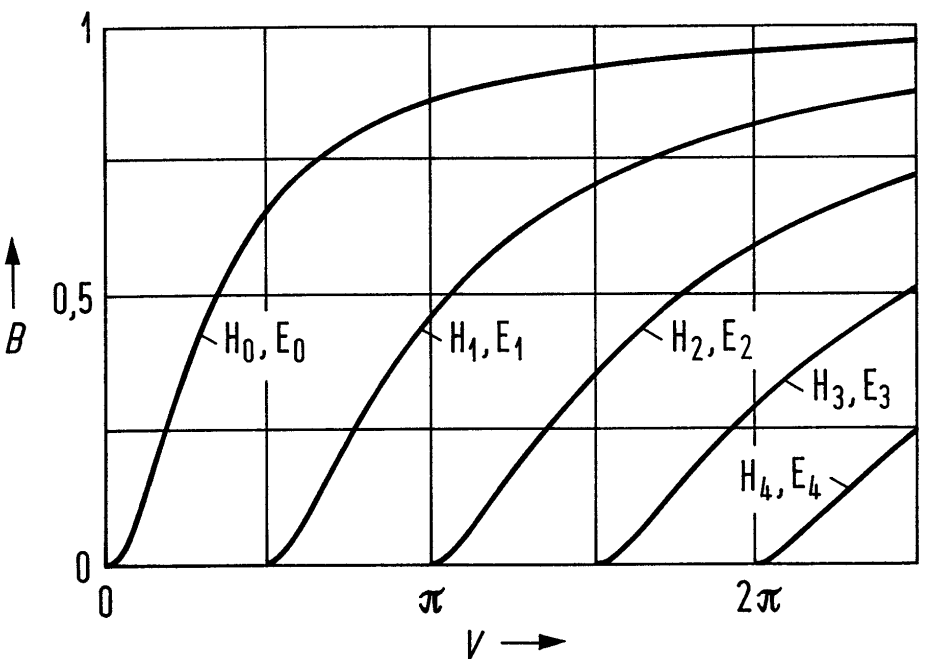
\includegraphics[width=.5\columnwidth]{Grafiken/SingleMode.png}%
\caption{Normalized propagation $B$ over normalized frequency $V$.}%
\label{fig:singlemoded}%
\end{figure}
To achieve a single mode strip waveguide the normalized frequency $V$ needs to be smaller than $\pi/2$. This can be explained by looking at the dispersion relation in Figure \ref{fig:singlemoded}\footnote[1]{Wolfgang Freude, Optische Wellenleiter und Sender, Lecture Notes}. For a normalized frequency $V$ a modes with the corresponding normalized wavenumber $B$ are guided. The normalized frequency calculates as:
\begin{equation}
V=ak_0\sqrt{n_1^2-n_2^2}
\label{eq:norm_freq}
\end{equation}
with $2a$ is the thickness of the core, $n_1$ is the refractive index of the core, $n_2$ is the refractive index of the cladding and $k_0 = 2\pi/\lambda$ is the wavenumber. Thus the parameters which determine the number of modes in a waveguide are the thickness of the core layer $2a$, the wavelength $\lambda$ and the refractive indices of the waveguide materials. For $V < \pi/2$ only the fundamental mode is guided. Note that there are still two polarizations H$_0$ and E$_0$.






\todo{wir ham nen asymetrischen waveguide angenommen, das bild is f�r symetrisch}
For the in \ref{q1} values assumed for $n_1$ and $n_2$ this leads to a core-thickness of
\begin{equation}
2a>\frac{\pi}{k_0\sqrt{n_1^2-n_2^2}}=\frac{\lambda_0}{2\sqrt{n_1^2-n_2^2}}=VALUE
\label{eq:}
\end{equation}
for $\lambda_0$ = 1550~nm.
